\documentclass[runningheads]{llncs}

\usepackage[T1]{fontenc}
\usepackage[utf8]{inputenc}
\usepackage[spanish,es-noquoting,es-noshorthands]{babel}
\usepackage{graphicx}
\usepackage{setspace}
\usepackage{hyperref}
\usepackage{listings}
\usepackage{geometry}
\usepackage{booktabs}
\usepackage[automake=delayed]{glossaries}
\usepackage[backend=biber,style=apa]{biblatex}
\usepackage{csquotes}

\usepackage[dvipsnames]{xcolor}

\hypersetup{
    hidelinks,
    colorlinks=false
}

\newcounter{glsnum}
\setcounter{glsnum}{0}

\renewcommand*{\glstextformat}[1]{
  \begin{NoHyper}#1\end{NoHyper}%
  \nobreak\hspace{0pt}%
  \stepcounter{glsnum}%
  \hyperlink{glo:\glslabel}{\textsuperscript{\textcolor{MidnightBlue}{\theglsnum}}}%
}

\onehalfspacing

\lstset{
    basicstyle=\ttfamily\footnotesize,
    breaklines=true,
    breakatwhitespace=true,
    frame=lines,
    captionpos=b,
    keywordstyle=\color{blue},
    commentstyle=\color{gray},
    stringstyle=\color{green!50!black},
    showstringspaces=false,
    literate={á}{{\'a}}1 {é}{{\'e}}1 {í}{{\'i}}1 {ó}{{\'o}}1 {ú}{{\'u}}1 {ñ}{{\~n}}1 {Á}{{\'A}}1 {É}{{\'E}}1 {Í}{{\'I}}1 {Ó}{{\'O}}1 {Ú}{{\'U}}1 {Ñ}{{\~N}}1
}

\makeglossaries

\addbibresource{references.bib}

% Dejar que el título del glosario lo gestione manualmente el documento (TOC numerado).
\setglossarysection{none}

\newglossaryentry{oidc}{
    name={OIDC},
    description={OpenID Connect. Capa de identidad basada en el protocolo OAuth 2.0 que permite a los clientes verificar la identidad de una entidad.}
}

\newglossaryentry{secretsprawl}{
    name={Secret Sprawl},
    description={Dispersión descontrolada de credenciales (claves API, certificados, tokens) a lo largo del ciclo de vida del desarrollo de software.}
}

\newglossaryentry{zerotrust}{
    name={Zero Trust},
    description={Modelo de ciberseguridad que asume que no existe confianza implícita concedida a los activos o cuentas basándose únicamente en su ubicación física o de red.}
}

\newglossaryentry{iac}{
    name={IaC},
    description={Infraestructura como Código. Gestión y aprovisionamiento de la infraestructura a través de código y manifiestos declarativos en lugar de procesos manuales.}
}

\newglossaryentry{cicd}{
    name={CI/CD},
    description={Integración Continua y Despliegue Continuo. Práctica de automatización que integra el desarrollo y el despliegue de software de forma constante y segura.}
}

\newglossaryentry{sdlc}{
    name={SDLC},
    description={Software Development Life Cycle (Ciclo de Vida del Desarrollo de Software). Proceso integral para el diseño, desarrollo, pruebas y despliegue de software de alta calidad.}
}

\newglossaryentry{ttl}{
    name={TTL},
    description={Time To Live (Tiempo de Vida). Período de validez o caducidad asignado a un recurso, como un token o una credencial efímera, antes de ser revocado automáticamente.}
}

\newglossaryentry{jwt}{
    name={JWT},
    description={JSON Web Token. Estándar abierto (RFC 7519) que define un modo compacto y autónomo para transmitir información de forma segura entre las partes como un objeto JSON.}
}

\newglossaryentry{mtls}{
    name={mTLS},
    description={Mutual Transport Layer Security. Proceso en el que ambas partes de una conexión de red autentican mutuamente sus certificados criptográficos.}
}

\newglossaryentry{siem}{
    name={SIEM},
    description={Security Information and Event Management. Sistema centralizado que proporciona análisis en tiempo real de alertas de seguridad generadas por el hardware y las aplicaciones de red.}
}

\newglossaryentry{hcl}{
    name={HCL},
    description={HashiCorp Configuration Language. Lenguaje declarativo utilizado para definir la infraestructura en herramientas como Terraform.}
}

\newglossaryentry{castillofoso}{
    name={Castillo y Foso},
    description={Modelo de seguridad perimetral tradicional basado en la premisa de defender una red interna segura mediante barreras externas, como firewalls. Asume que los usuarios y dispositivos dentro del perímetro son de confianza, un enfoque que resulta ineficaz en entornos distribuidos modernos.}
}

\newglossaryentry{sast}{
    name={SAST},
    description={Static Application Security Testing. Análisis del código fuente en busca de vulnerabilidades aplicando reglas estáticas antes de la ejecución.}
}

\newglossaryentry{dast}{
    name={DAST},
    description={Dynamic Application Security Testing. Pruebas de seguridad sobre una aplicación en ejecución para identificar vulnerabilidades mediante interacciones y análisis dinámico.}
}

\newglossaryentry{iast}{
    name={IAST},
    description={Interactive Application Security Testing. Combinación de técnicas de análisis dinámico e instrumentación en tiempo de ejecución para detectar vulnerabilidades con contexto.}
}

\newglossaryentry{mfa}{
    name={MFA},
    description={Multi-Factor Authentication. Autenticación que exige dos o más factores (p. ej., algo que eres, algo que tienes, algo que sabes).}
}

\newglossaryentry{policyascode}{
    name={Policy-as-Code},
    description={Modelo que codifica políticas de seguridad como artefactos versionados y ejecutables automáticamente para aplicar controles consistentes.}
}

\newglossaryentry{cli}{
    name={CLI},
    description={Command-Line Interface. Interfaz de línea de comandos para operar herramientas y automatizar tareas.}
}

\newglossaryentry{vault}{
    name={Vault},
    description={HashiCorp Vault. Bóveda que gestiona secretos y credenciales con cifrado, control de acceso y generación dinámica según políticas.}
}

\newglossaryentry{lxc}{
    name={LXC},
    description={Linux Containers. Tecnología de contenedores basada en aislamiento a nivel de sistema operativo en Linux.}
}

\newglossaryentry{kubernetes}{
    name={Kubernetes},
    description={Plataforma de orquestación de contenedores que automatiza despliegue, escalado y operación de aplicaciones.}
}

\newglossaryentry{k3s}{
    name={k3s},
    description={Distribución ligera de Kubernetes, diseñada para simplificar la instalación y operación en entornos con recursos limitados.}
}

\newglossaryentry{raft}{
    name={Raft},
    description={Algoritmo de consenso utilizado para replicación y mantenimiento de estado en sistemas distribuidos (p. ej., motores de almacenamiento en Vault).}
}

\newglossaryentry{tls}{
    name={TLS},
    description={Transport Layer Security. Protocolo criptográfico para proteger comunicaciones en redes.}
}

\setcounter{tocdepth}{3}
\setcounter{secnumdepth}{3}

\begin{document}

\title{MÁSTER EN CIBERSEGURIDAD \\ \vspace{0.5cm} \large MÓDULO 11. TRABAJO FIN DE MÁSTER (TFM)}
\subtitle{La Crisis de la Gestión de Secretos: Secret Sprawl}

\author{Andrea Osma Rafael}
\institute{Campus de Ciberseguridad}

\titlerunning{TFM Ciberseguridad - Secret Sprawl}
\authorrunning{A. Osma Rafael}

\pagenumbering{gobble} 
\maketitle

\begin{abstract}
TFM del Máster de Ciberseguridad de la ENIIT sobre la problemática del \gls{secretsprawl} en entornos DevSecOps. Se analiza la fuga de credenciales en repositorios y pipelines de \gls{cicd}, proponiendo una arquitectura basada en bóvedas criptográficas y gestión dinámica de identidades.
\keywords{Ciberseguridad \and DevSecOps \and Secret Sprawl \and Gestión de Secretos \and Zero Trust}
\end{abstract}

\newpage

\addtocontents{toc}{\protect\setcounter{tocdepth}{3}} % Opcional: limita profundidad en el índice si es muy largo
\pagenumbering{arabic} 
\tableofcontents
\newpage

\section{Estado del Arte}
\subsection{Introducción: El Colapso del Perímetro Tradicional}

La evolución de la infraestructura IT, desde los centros de datos locales hacia la computación en la nube y las arquitecturas de microservicios, ha forzado una reevaluación total de los modelos de confianza. El modelo de seguridad perimetral, basado en la premisa de una red interna segura protegida por firewalls (Castillo y Foso), ha demostrado ser ineficaz en entornos donde las cargas de trabajo son efímeras y se distribuyen en múltiples nubes.

\subsubsection{El Paradigma Zero Trust y el Cumplimiento Normativo}
Según la publicación especial NIST SP 800-207, la Arquitectura \gls{zerotrust} (ZTA) es un modelo de ciberseguridad que asume que no existe confianza implícita concedida a los activos o cuentas de usuario basándose únicamente en su ubicación física o de red. En lugar de defender un perímetro estático, la autenticación y autorización se evalúan de forma dinámica y continua por cada solicitud de acceso, protegiendo los recursos de manera individualizada \parencite{nist_sp800_207}.

A nivel regulatorio, este cambio de paradigma se ha materializado en marcos europeos recientes como la directiva NIS2 y DORA (Digital Operational Resilience Act). Estas normativas exigen a las organizaciones, especialmente en infraestructuras críticas y el sector financiero, implementar controles estrictos y demostrables sobre la gestión de identidades, la resiliencia operativa y el riesgo de la cadena de suministro. La rotación automatizada de credenciales y la auditoría continua pasan de ser buenas prácticas a ser obligaciones legales estrictas \parencite{nis2_2022_2555,dora_2022_2554}.

En el paradigma actual, la red es dinámica y, por definición, hostil. Por tanto, la seguridad debe desplazarse desde la red hacia la identidad. Este cambio sitúa a la Gestión de Identidad y Acceso (IAM) no como un servicio de soporte, sino como el plano de control central de la seguridad de la información. Este TFM analiza soluciones diseñadas para mitigar los riesgos derivados de la proliferación de identidades no humanas.

\subsection{La Crisis de la Gestión de Secretos: Secret Sprawl}

\subsubsection{Taxonomía de la Dispersión de Secretos}

El término \gls{secretsprawl} define la distribución descontrolada de credenciales (claves API, certificados, tokens, contraseñas) a lo largo del ciclo de vida del desarrollo de software (\gls{sdlc}). En un entorno de Infraestructura como Código (\gls{iac}), el riesgo aumenta considerablemente.

\begin{itemize}
    \item \textbf{Fugas en Control de Versiones:} La inmutabilidad de los sistemas como Git implica que un secreto subido accidentalmente persiste en el historial, requiriendo un proceso complejo de rewriting history o la invalidación inmediata de la credencial.
    \item \textbf{Variables de Entorno Inseguras:} El uso de archivos .env o variables de sistema sin cifrar en servidores de \gls{cicd} (Jenkins, GitHub Actions) expone credenciales a cualquier proceso con privilegios de lectura en el entorno.
    \item \textbf{Certificados X.509 y Claves SSH Compartidas:} La emisión de certificados de larga duración o el uso de pares de claves SSH estáticas sin el respaldo de una Autoridad de Certificación (CA) efímera provoca que, si el material privado es comprometido, el acceso se mantenga de forma prolongada sin ser detectado.
    \item \textbf{Credenciales Hardcodeadas en Código Fuente:} La práctica de incrustar tokens o contraseñas directamente en los repositorios expone la información a cualquier usuario con privilegios de lectura y propaga el secreto a través de los artefactos de construcción.
\end{itemize}

\subsubsection{El Desafío de la Escala: Máquinas vs. Humanos}

Investigaciones recientes sugieren que las identidades de máquinas (servicios, contenedores, bots) crecen a un ritmo cinco veces superior al de las identidades humanas. A diferencia de un operador humano, que puede validar su identidad aportando biometría o un token de hardware en un flujo \gls{mfa} tradicional, una carga de trabajo automatizada carece de este factor interactivo ("algo que eres" o "algo que tienes").

Esto exige sustituir el \gls{mfa} humano por la validación concurrente de múltiples atributos criptográficos y contextuales. Se requiere la presentación de credenciales como certificados \gls{tls} mutuos (\gls{mtls}) o tokens \gls{jwt} firmados, combinados con la verificación de la IP de origen, el namespace o la rama del repositorio en tiempo de ejecución. Se espera que la validación estricta de estos metadatos limite la emisión de secretos exclusivamente a las cargas de trabajo legítimas \parencite{rfc7519_jwt}.

\subsubsection{Riesgos de Seguridad Derivados del Secret Sprawl}
El almacenamiento incontrolado y la exposición de credenciales generan vectores de ataque críticos en las infraestructuras modernas. La literatura académica señala que la exposición de secretos en pipelines de \gls{cicd} y en repositorios de código facilita la ejecución de los siguientes escenarios de compromiso:

\begin{itemize}
    \item \textbf{Movimiento Lateral y Escalada de Privilegios:} En arquitecturas planas o basadas en microservicios, un atacante que obtiene un token de acceso básico puede pivotar hacia sistemas críticos o bases de datos si no existe una autenticación estricta.
    \item \textbf{Ataques a la Cadena de Suministro (Supply Chain Attacks):} La inyección de código malicioso en los flujos de integración continua a menudo se logra explotando credenciales expuestas en los repositorios, lo que compromete las fases de construcción y despliegue del software de forma automatizada.
    \item \textbf{Persistencia a Largo Plazo:} Las credenciales estáticas que carecen de rotación permiten a los atacantes mantener un acceso indetectable a la infraestructura (comportamiento esperado tras una intrusión exitosa), incluso después de que los equipos de respuesta a incidentes mitiguen la vulnerabilidad técnica inicial que permitió la entrada.
\end{itemize}

\subsubsection{El Ciclo de Vida del Secreto}

Para mitigar los riesgos asociados a la dispersión de credenciales, la gestión de secretos debe tratarse como un proceso continuo e integrado. Los secretos se consideran artefactos de primer nivel que requieren un ciclo de vida definido desde su creación hasta su destrucción. Este ciclo consta de las siguientes fases:

\begin{enumerate}
    \item \textbf{Generación:} Creación de la credencial, preferiblemente de forma dinámica y asociando un Tiempo de Vida (\gls{ttl}) estrictamente limitado a la misma.
    \item \textbf{Almacenamiento Seguro:} Custodia del secreto en un almacén centralizado que proporcione cifrado y aplique controles de acceso basados en políticas (\gls{policyascode}) para definir quién, y bajo qué condiciones, puede interactuar con el dato.
    \item \textbf{Distribución e Inyección:} Entrega temporal del secreto a la identidad que lo solicita (humana o de máquina) en tiempo de ejecución, evitando en todo momento su escritura en disco.
    \item \textbf{Rotación:} Renovación periódica o basada en eventos de las credenciales, un proceso fundamental para invalidar versiones anteriores y acotar drásticamente la ventana de exposición ante una posible brecha.
    \item \textbf{Revocación y Auditoría:} Invalidación del secreto en el sistema de destino tras expirar su \gls{ttl}, manteniendo un registro inmutable de todas las operaciones para facilitar labores de cumplimiento normativo y diagnóstico forense.
\end{enumerate}

\subsubsection{Integración Transversal en el SDLC (DevSecOps)}

La gestión de identidades y secretos interactúa a lo largo de todo el Ciclo de Vida del Desarrollo de Software (\gls{sdlc}). Aplicar el principio de shift-left security exige implementar controles técnicos desde las fases más tempranas:

\begin{itemize}
    \item \textbf{Fase de Código (Code and Commit):} Constituye la primera línea de defensa. Dado que es habitual que se introduzcan credenciales hardcodeadas de manera inadvertida, en esta etapa se despliegan escaneos de secretos y hooks de pre-commit en los repositorios locales para bloquear la inyección en el control de versiones \parencite{owasp_secrets_management_cheat_sheet,github_secret_scanning}.
    \item \textbf{Fase de Construcción (Build and CI):} Los servidores de Integración Continua requieren acceso a repositorios de artefactos y entornos de prueba. El uso de variables de entorno estáticas en esta fase representa un riesgo significativo de fuga de datos. Los secretos deben ser inyectados dinámicamente y enmascarados para evitar su volcado accidental en los registros (logs) de ejecución.
    \item \textbf{Fase de Pruebas (Test):} Las herramientas de análisis dinámico e interactivo (\gls{dast} e \gls{iast}) necesitan credenciales temporales para ejecutar sus escaneos en los entornos de validación. Esta fase garantiza la separación estricta entre las credenciales de prueba y las de producción.
    \item \textbf{Fase de Despliegue y Operación (Deploy and Run):} En la etapa final, las cargas de trabajo contenerizadas u orquestadas solicitan sus credenciales en tiempo de ejecución. El gestor central valida la identidad criptográfica de la carga de trabajo y entrega un acceso efímero vinculado a políticas contextuales.
\end{itemize}

\subsection{Trazabilidad Forense y Dispositivos de Auditoría}
Un pilar fundamental de la Arquitectura \gls{zerotrust} es la visibilidad total sobre las peticiones de acceso. Durante las pruebas, se habilitó el motor de auditoría de \gls{vault} para registrar cada interacción en formato JSON. Este registro inmutable captura el identificador de la entidad solicitante, la política evaluada, la ruta del secreto y la marca de tiempo exacta \parencite{vault_audit_devices}.

La exportación de estos registros estructurados hacia un sistema \gls{siem} centralizado permite la detección de anomalías en tiempo real, como múltiples intentos de acceso denegados desde una IP específica, garantizando así los requisitos de resiliencia y auditoría continua exigidos por marcos normativos actuales.

\section{Motivación}

La transición de arquitecturas monolíticas a ecosistemas distribuidos, contenerizados y orientados a microservicios ha redefinido radicalmente el perímetro de seguridad clásico. En este paradigma actual, la red subyacente se asume como un entorno intrínsecamente hostil, desplazando a la identidad hacia el centro del plano de control. Este avance arquitectónico, si bien ha dotado de agilidad al desarrollo, ha precipitado una crisis operativa sin precedentes: la proliferación descontrolada de identidades no humanas, tales como servicios, contenedores y automatizaciones de despliegue. A diferencia de los usuarios humanos, estas entidades requieren mecanismos de autenticación criptográfica automatizados y de alta frecuencia, lo que ha derivado en el fenómeno conocido como \gls{secretsprawl} (dispersión de secretos) a lo largo del ciclo de vida del desarrollo de software (\gls{sdlc}).

En paralelo, la consolidación de las metodologías ágiles ha convertido a los repositorios de código y a las plataformas de Integración y Despliegue Continuo (\gls{cicd}) en la columna vertebral de la ingeniería de software y, consecuentemente, en vectores de ataque de alto valor. La persistencia técnica de incrustar credenciales estáticas (hardcoding) o de utilizar variables de entorno debilmente protegidas expone a las infraestructuras a riesgos severos, facilitando el movimiento lateral y el compromiso de la cadena de suministro. Este escenario se vuelve críticamente complejo en sectores sometidos a estrictas normativas (como defensa, banca o infraestructuras críticas), donde la soberanía del dato exige despliegues en nubes privadas (on-premise) fuertemente aisladas. Históricamente, la innovación en la inyección dinámica de credenciales se ha diseñado de forma nativa para la nube pública, dejando a las infraestructuras locales relegadas a prácticas heredadas y a un control perimetral obsoleto.

La gestión manual de material criptográfico, como la rotación de contraseñas o la renovación de certificados X.509, no solo introduce una carga operativa severa para los equipos de ingeniería, sino que también incrementa la probabilidad de interrupciones del servicio debido a errores humanos u omisiones.

La motivación fundamental de este proyecto es cerrar esta brecha tecnológica, demostrando la viabilidad de integrar los más altos estándares de seguridad y gestión de identidad efímera en entornos privados restrictivos. Se busca evidenciar que la adopción de una cultura DevSecOps genuina donde la seguridad se codifica e inyecta en las fases iniciales del desarrollo (shift-left) permite sustituir los secretos estáticos por flujos de autenticación dinámicos bajo demanda. Al abstraer toda esta arquitectura mediante herramientas de Infraestructura como Código (\gls{iac}), se persigue establecer un modelo operativo inmutable y auditable desde la línea de comandos. Esta aproximación técnica pretende sentar las bases para una migración interoperable hacia arquitecturas de nube híbrida, estandarizando los controles de acceso independientemente del hipervisor o proveedor subyacente.

\section{Hipótesis}

La presente investigación plantea que la integración de una arquitectura de seguridad centrada en la identidad, materializada a través de una bóveda criptográfica centralizada, reduce sustancialmente la superficie de ataque en entornos de nube privada sujetos a estrictos requisitos de soberanía del dato y aislamiento. Al transicionar de un modelo de confianza perimetral estático a un enfoque anclado en los principios de \gls{zerotrust}, donde la inyección de credenciales se realiza de forma dinámica y estrictamente bajo demanda, se espera que la ventana de oportunidad para la explotación de credenciales comprometidas se acote drásticamente frente a ataques automatizados.

Asimismo, se hipotetiza que la inserción de controles de seguridad de forma transversal (\gls{sast}, \gls{dast} y análisis de composición de software) directamente en el pipeline de Integración y Despliegue Continuo (\gls{cicd}) madura la postura de seguridad del ciclo de vida del software. Retirar el material criptográfico persistente del código fuente y de los repositorios de control de versiones mitiga el riesgo de \gls{secretsprawl} y dificulta el movimiento lateral o la escalada de privilegios en caso de una intrusión inicial.

Finalmente, desde el punto de vista de la ingeniería de la infraestructura, se postula que la orquestación de este ecosistema mediante paradigmas de Infraestructura como Código (\gls{iac}) desvinculando la capa de gestión de acceso de la topología de red subyacente proporciona la abstracción necesaria para escalar el modelo operativo. El uso de manifiestos declarativos y automatización modular facilita la exportación de esta misma arquitectura desde un entorno on-premise virtualizado hacia un modelo de nube híbrida pública, manteniendo la cohesión y las políticas de seguridad inmutables sin requerir una reingeniería profunda de la lógica de acceso.


\section{Tesis: Arquitectura DevSecOps para la Gestión Dinámica de Secretos}

La propuesta central de este proyecto consiste en el diseño e implementación de una arquitectura centralizada de gestión de secretos, fundamentada en el paradigma \gls{zerotrust}. El objetivo principal es la sustitución de credenciales estáticas por flujos de inyección dinámica, orquestados íntegramente mediante Infraestructura como Código (\gls{iac}).

\subsection{Diseño de la Arquitectura Lógica}
El núcleo del sistema reside en una bóveda criptográfica de alta disponibilidad (como HashiCorp \gls{vault}), configurada para operar como la única fuente de verdad para el material sensible. La arquitectura se segmenta en tres planos funcionales:

\begin{itemize}
    \item \textbf{Plano de Autenticación:} Las cargas de trabajo (contenedores, pipelines de despliegue) no poseen secretos iniciales estáticos en disco. Se autentican contra la bóveda utilizando identidades nativas de su entorno de ejecución, tales como tokens \gls{jwt} en entornos de \gls{cicd} mediante \gls{oidc} (OpenID Connect) o Service Accounts en orquestadores \parencite{rfc7519_jwt,oidc_core_1_0}.
    \item \textbf{Plano de Autorización:} Una vez autenticada la entidad no humana, un motor de políticas (\gls{policyascode}) evalúa de forma estricta si la identidad posee los privilegios mínimos necesarios para acceder a la ruta del secreto solicitado.
    \item \textbf{Plano de Emisión Dinámica:} En lugar de devolver una credencial de larga duración, el sistema genera credenciales efímeras bajo demanda (por ejemplo, usuarios temporales de bases de datos o certificados de corta duración) con un Tiempo de Vida (\gls{ttl}) ajustado al tiempo de ejecución de la tarea.
\end{itemize}

\subsection{Resolución del Problema del "Secreto Cero" (Secret Zero)}
El desafío técnico más complejo en la automatización de secretos es el método para entregar el primer vector de autenticación a una máquina sin incurrir en prácticas de hardcoding. La solución propuesta aborda este dilema delegando la raíz de confianza en el proveedor de infraestructura subyacente. 

Al emplear federación de identidades (\gls{oidc}) para los flujos de integración continua, el pipeline presenta a la bóveda un token criptográfico firmado temporalmente por el proveedor de \gls{cicd}. La bóveda verifica la firma pública de este token frente a las claves públicas del proveedor. En consecuencia, el código fuente y los manifiestos de despliegue permanecen completamente limpios de material criptográfico persistente. Se espera que este diseño acote significativamente la superficie de exposición en los repositorios de código, si bien la integridad total depende de la robustez del proveedor de identidades externo, constituyendo un comportamiento esperado de mitigación, no una protección absoluta ante vulnerabilidades de terceros \parencite{oidc_core_1_0}.

\begin{figure}[htbp]
    \centering
    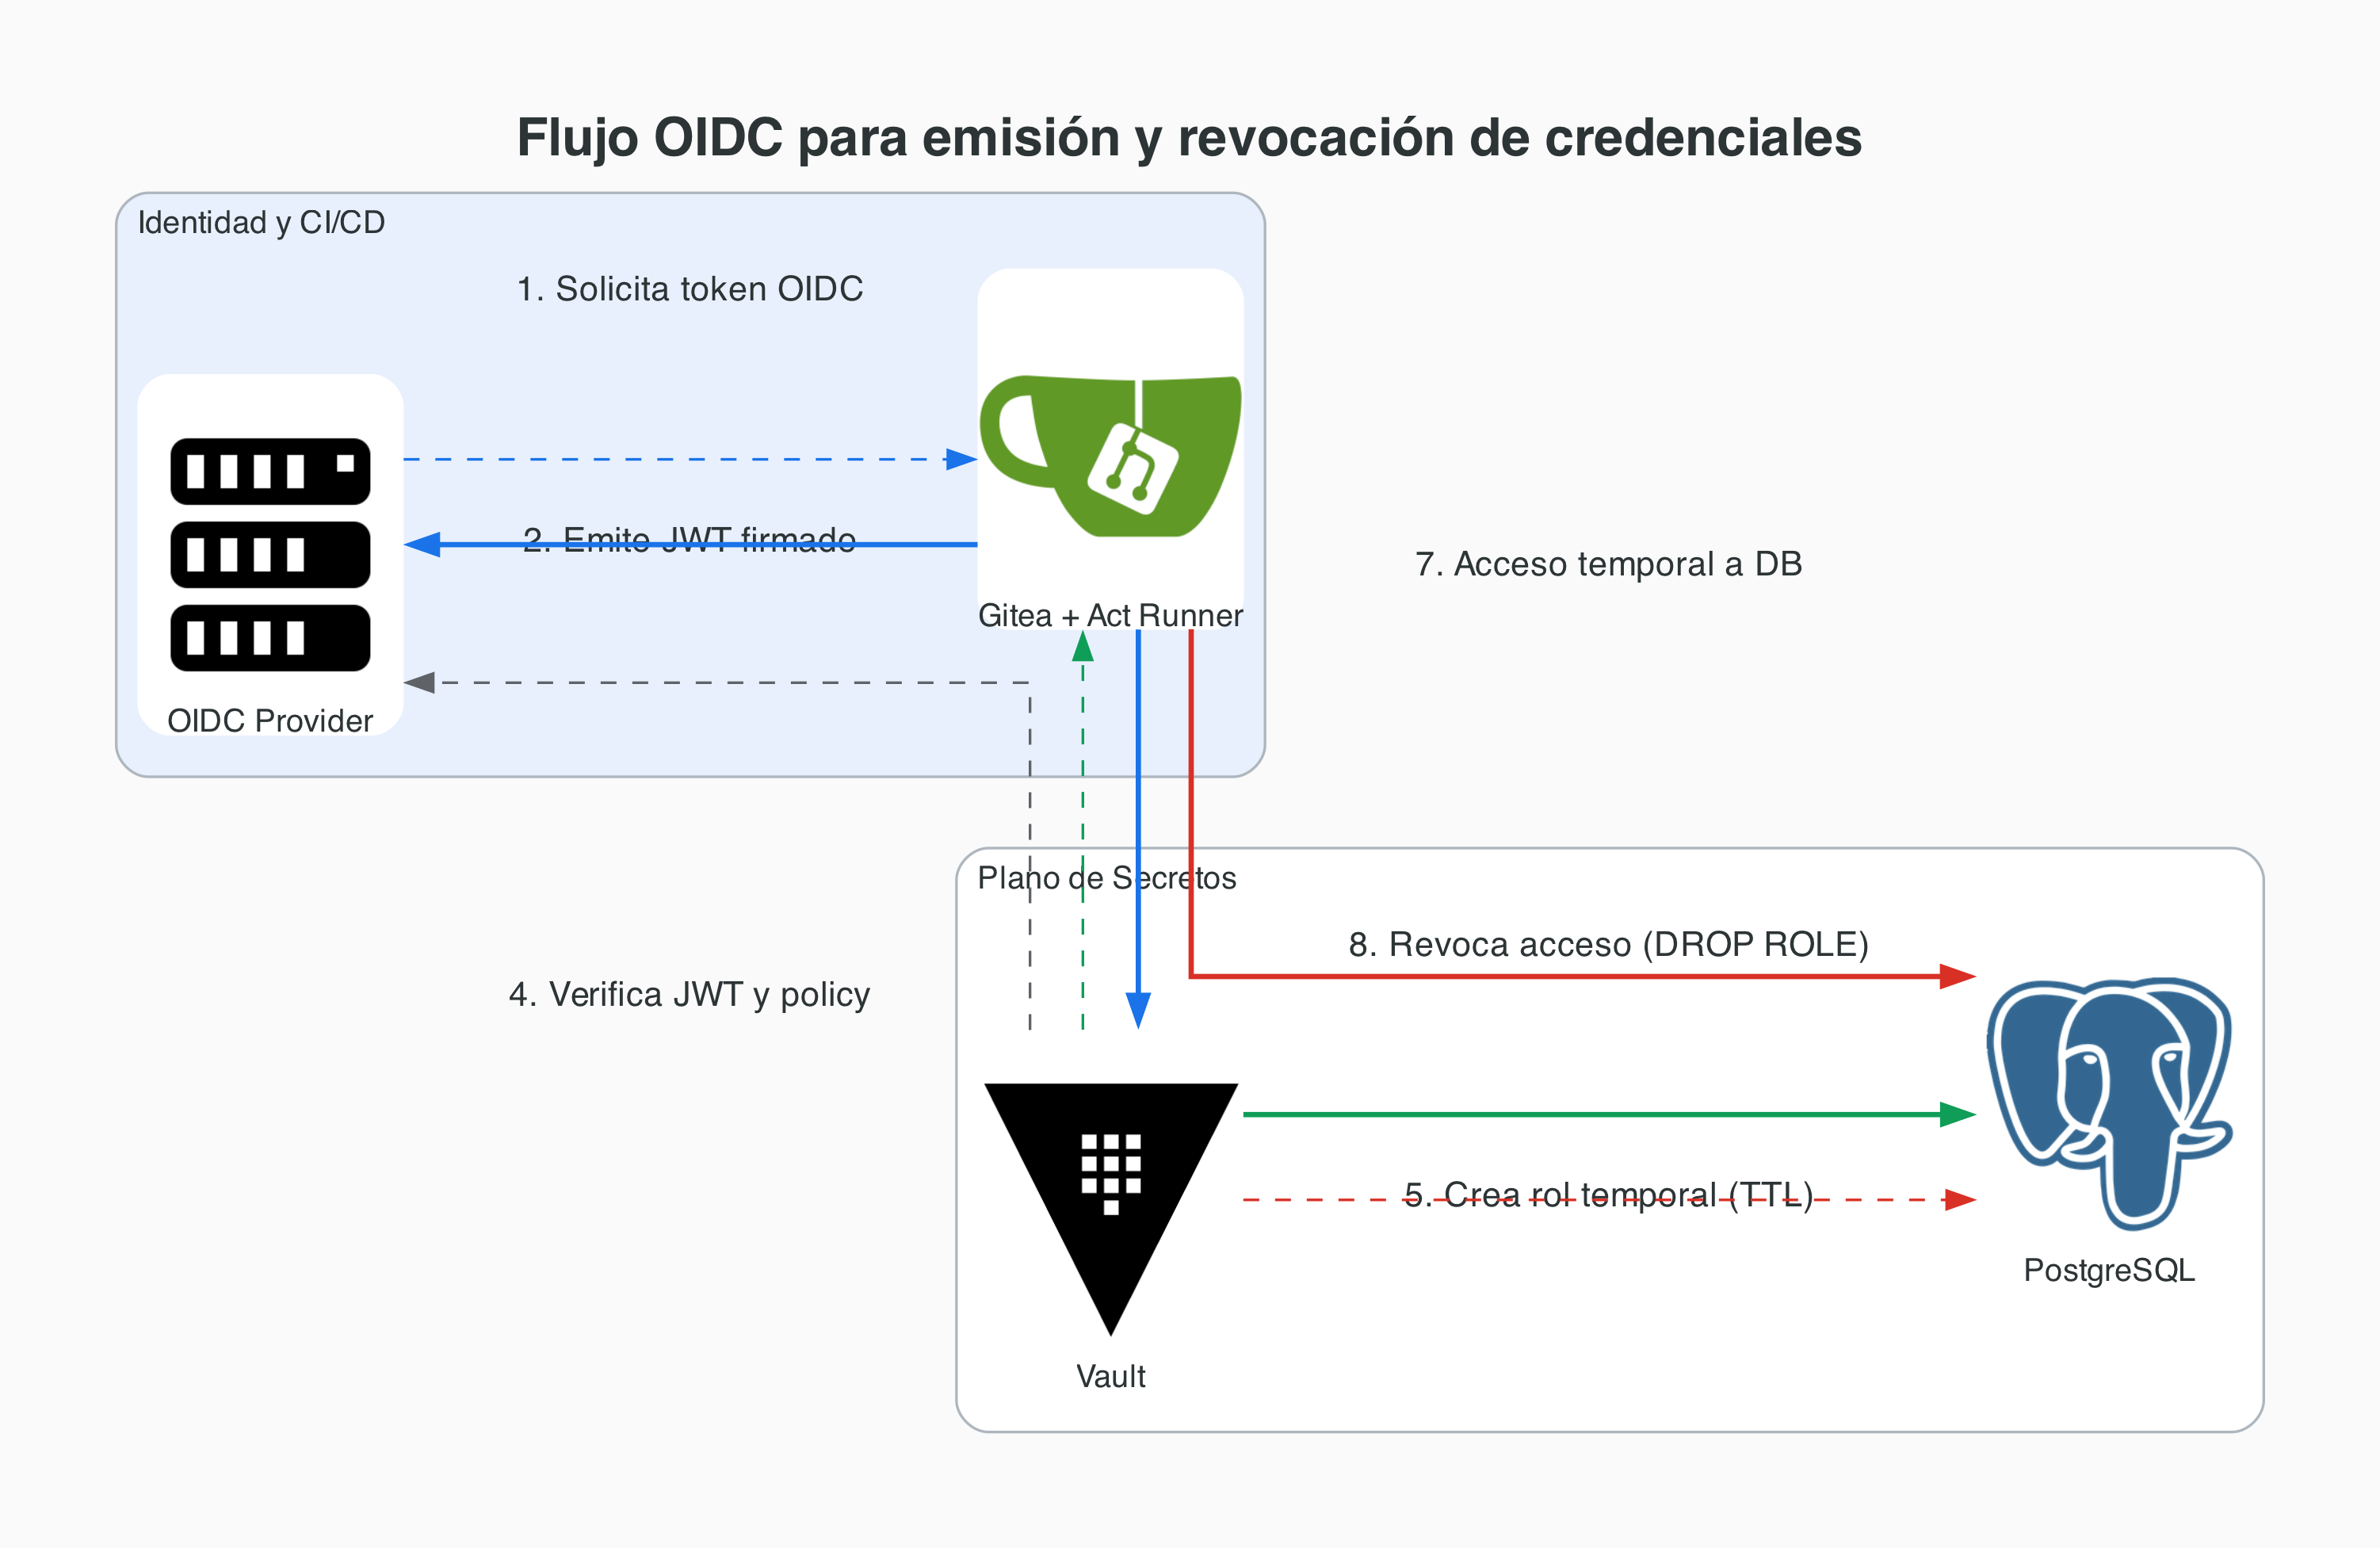
\includegraphics[width=\textwidth]{diagrams/flujo_oidc_secrets.png}
    \caption{Secuencia de autenticación federada mediante OIDC y emisión/revocación de credenciales efímeras en Vault para acceso temporal a PostgreSQL.}
    \label{fig:flujo-oidc-secrets}
\end{figure}

\subsection{Despliegue Inmutable y Operativa de Ingeniería}
La abstracción de toda la infraestructura y configuración de seguridad se define mediante manifiestos declarativos. La inicialización de la bóveda, la definición de roles y la asignación de políticas de acceso se gestionan como código, permitiendo un versionado estricto y un control de cambios mediante flujos de revisión. 

Fomentando una operativa técnica de alto rendimiento y reduciendo la fricción en la automatización, la interacción con el sistema en fases de administración e ingeniería se realiza exclusivamente mediante herramientas de interfaz de línea de comandos (\gls{cli}) y editores de terminal. Se descarta la dependencia de interfaces gráficas (GUI), lo que facilita la creación de scripts de automatización y establece un registro de comandos auditable para cada modificación en el estado de la seguridad. Es por este motivo que la arquitectura propuesta se despliega mediante Terraform \parencite{terraform_documentation}.

\section{Demostración}

\subsection{Entorno de Pruebas}
Para la validación empírica de la arquitectura propuesta, se ha desplegado un laboratorio \textit{on-premise} sobre un hipervisor tipo 1 (Proxmox VE 8.4.17). La infraestructura de hardware asignada consta de 48 GB de memoria RAM, un disco de estado sólido (SSD) de 256 GB para el almacenamiento operativo de alta velocidad gestionado mediante aprovisionamiento fino (\textit{thin provisioning}), y un disco duro mecánico (HDD) de 1 TB destinado a volcados de seguridad periódicos (\texttt{vzdump}).

La topología de red y computación se segmenta utilizando una combinación de contenedores Linux (\gls{lxc}) para servicios base y Máquinas Virtuales (VM) para la orquestación, distribuidos de la siguiente manera:

\begin{itemize}
    \item \textbf{\gls{lxc} 1 (Gitea v1.21 + Act Runner):} Plataforma ligera para el control de versiones y la ejecución de pipelines de \gls{cicd}, configurada para emitir tokens \gls{oidc}.
    \item \textbf{\gls{lxc} 2 (HashiCorp \gls{vault} v1.17.5):} Bóveda criptográfica central con motor de almacenamiento integrado (\gls{raft}) en configuración de nodo único.
    \item \textbf{\gls{lxc} 3 (PostgreSQL v17):} Motor de base de datos relacional que actúa como sistema objetivo para la inyección dinámica de credenciales.
    \item \textbf{VM 1 (\gls{k3s}, canal \textit{stable}; validado en v1.34.5+k3s1):} Clúster de \gls{kubernetes} ligero sobre una distribución Debian minimalista. El uso de una máquina virtual proporciona aislamiento a nivel de kernel, lo cual mitiga vectores de escape de contenedores \parencite{kubernetes_overview,k3s_documentation}.
\end{itemize}

\begin{figure}[htbp]
    \centering
    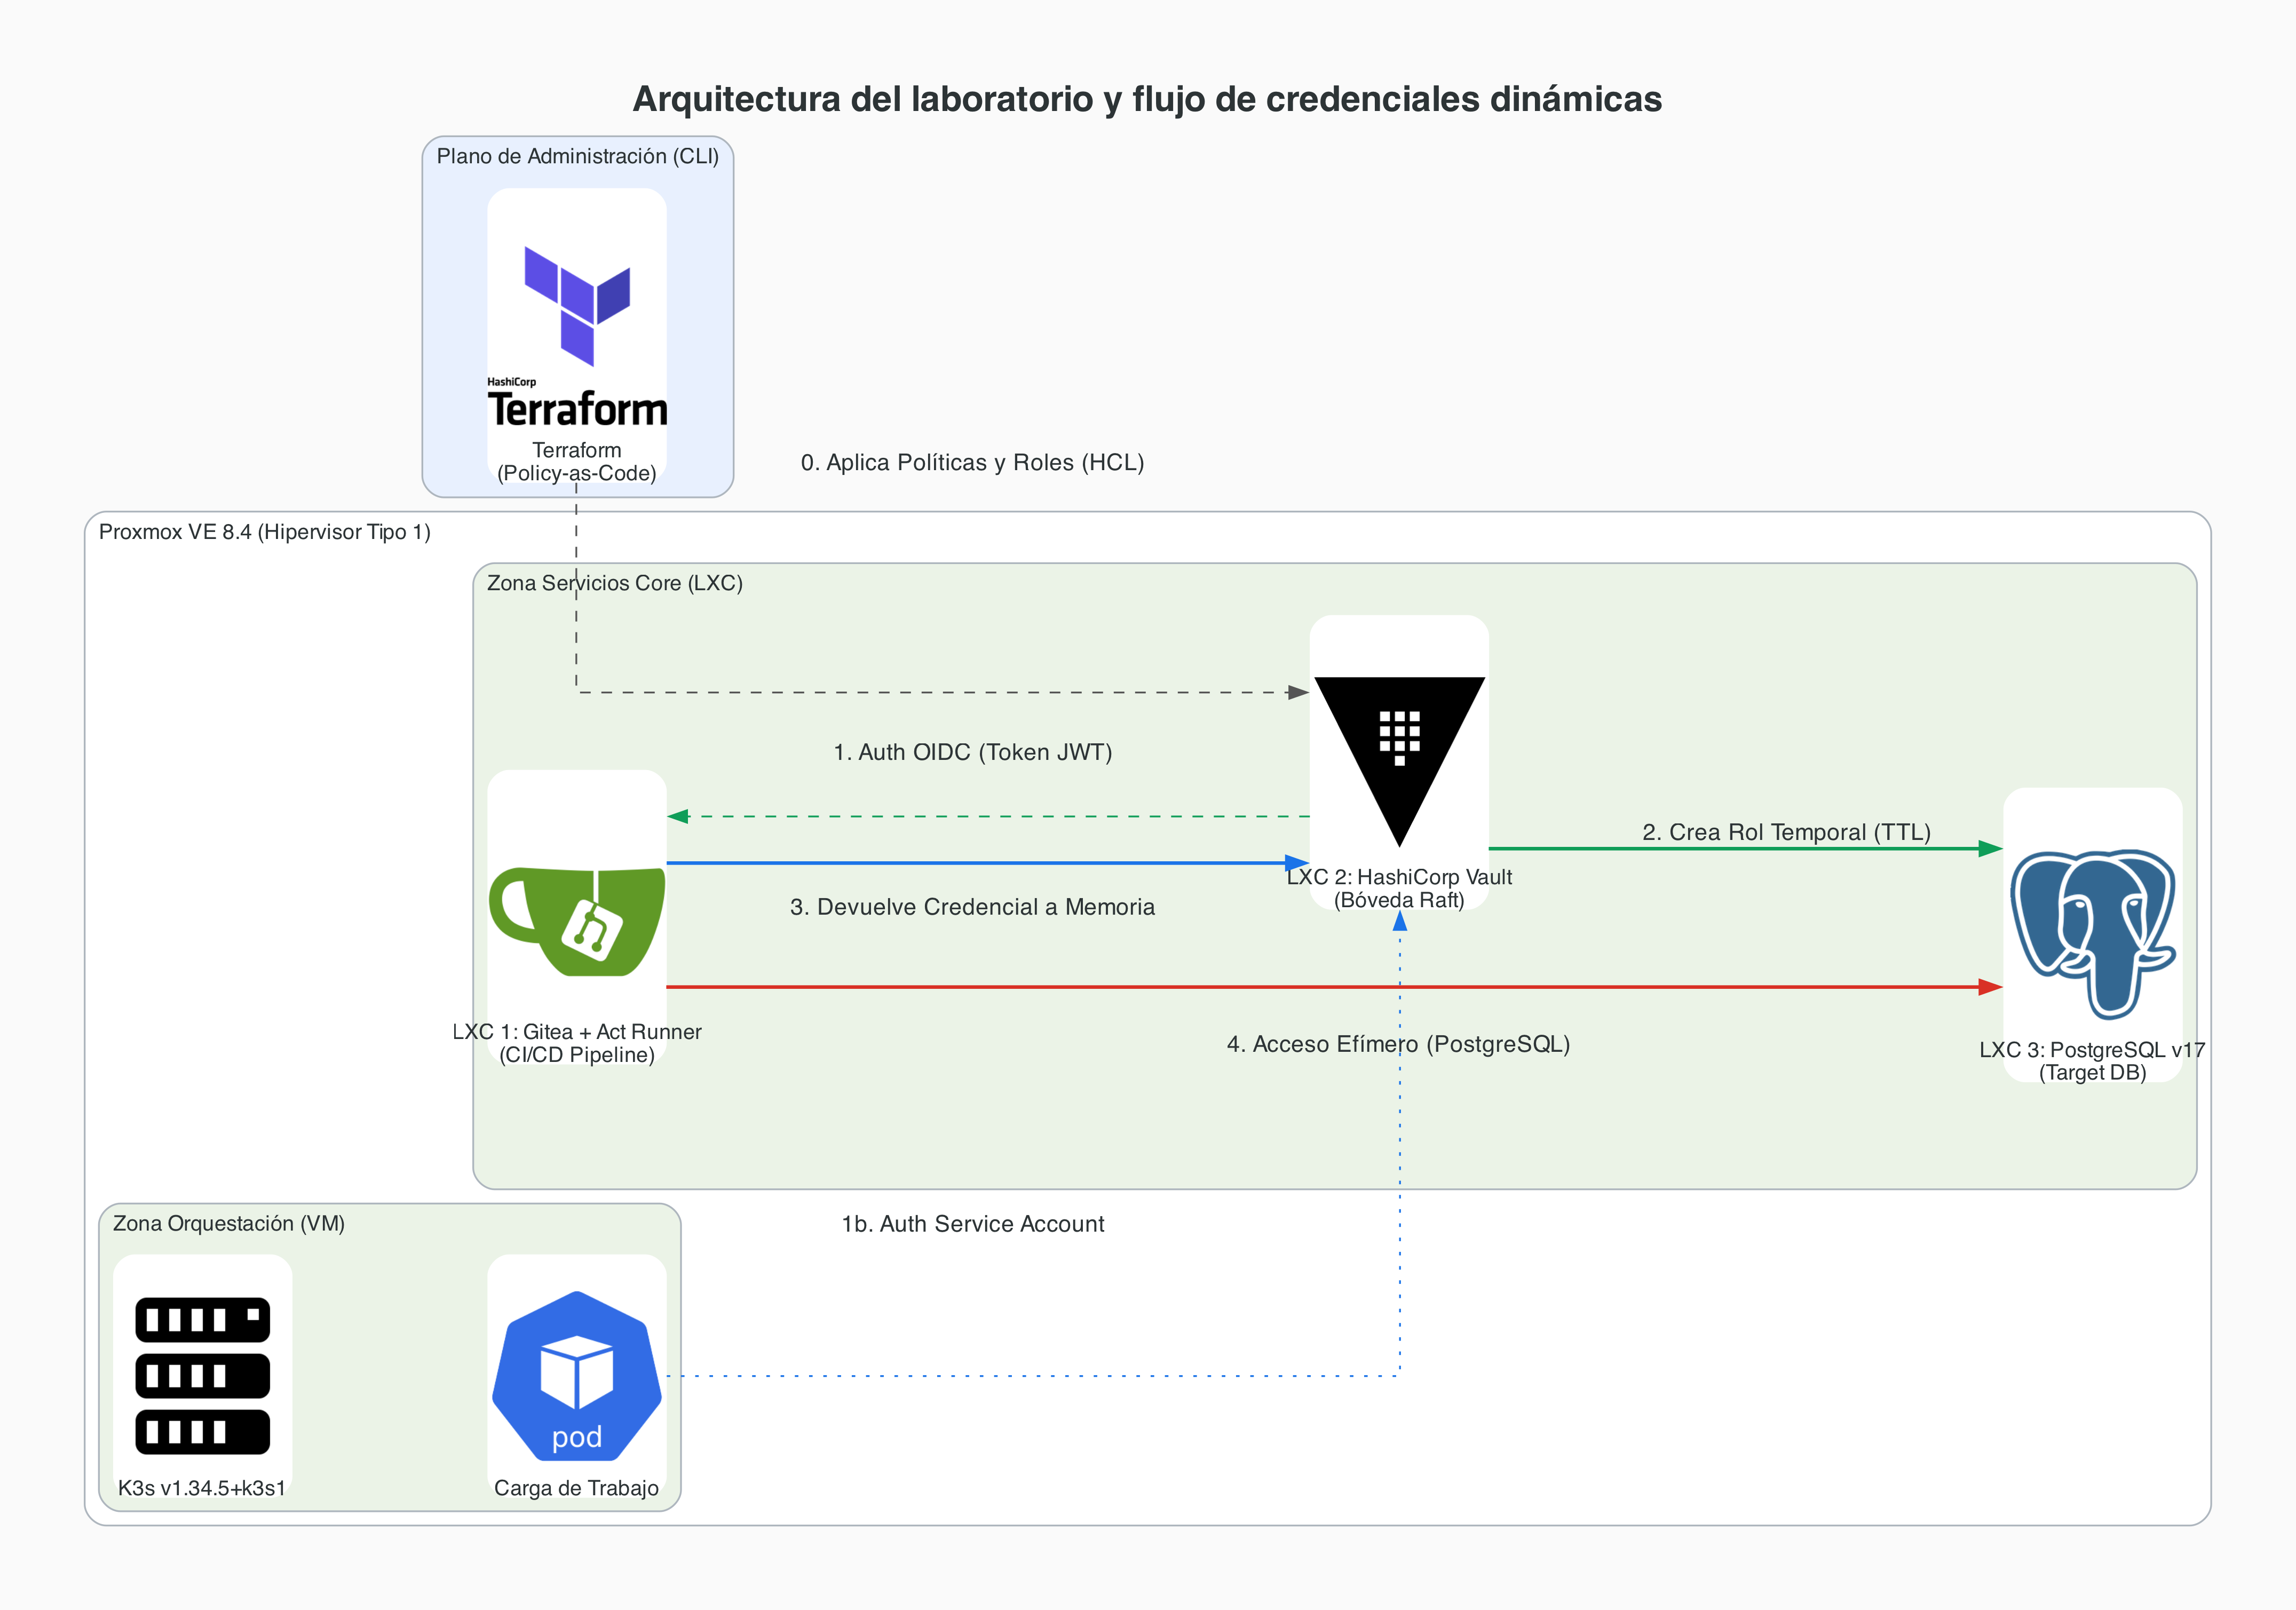
\includegraphics[width=\textwidth]{diagrams/topologia.png}
    \caption{Arquitectura DevSecOps y flujo de inyección dinámica de credenciales en el laboratorio \textit{on-premise}.}
    \label{fig:topologia}
\end{figure}

Fomentando una operativa técnica ágil, la administración del entorno y la configuración de políticas en \gls{vault} se realiza de forma exclusiva mediante su \gls{cli} y la edición de manifiestos con \texttt{vi}. Esto permite una integración natural con repositorios de Infraestructura como Código (\gls{iac}) y mantiene un registro de auditoría estricto, prescindiendo totalmente de interfaces gráficas \parencite{vault_audit_devices,terraform_documentation}.

\subsection{Estrategia de Despliegue mediante IaC}
La orquestación de la seguridad y el control de accesos se define íntegramente a través de archivos de configuración declarativos (\gls{hcl}) utilizando Terraform. Desde la terminal, mediante la edición de estos manifiestos, se establece la configuración del proveedor de HashiCorp \gls{vault}, la creación de políticas estructuradas (\gls{policyascode}) y la habilitación de los motores de secretos \parencite{terraform_documentation}.

Esta estrategia permite versionar la infraestructura de seguridad directamente en el repositorio de Gitea. Al aplicar los cambios de estado de forma determinista, se garantiza la inmutabilidad del entorno y se elimina la configuración manual.  Al prescindir de interfaces gráficas y operar exclusivamente mediante \gls{cli}, cualquier modificación en los roles o en los tiempos de vida (\gls{ttl}) de los secretos queda registrada en el control de versiones, habilitando un proceso de revisión por pares (Pull Requests) antes de su aplicación en producción \parencite{terraform_documentation}.

\subsubsection{Instalación de dependencias en Proxmox}
Para garantizar la reproducibilidad del entorno de laboratorio en el hipervisor Proxmox, la fase inicial del despliegue requiere la preparación del host. Este proceso se ha automatizado mediante un script de inicialización (\textit{shell script}) que estandariza las dependencias operativas antes de la ejecución de cualquier manifiesto declarativo.

El script cumple tres funciones críticas en la cadena de aprovisionamiento:

\begin{itemize}
    \item \textbf{Gestión de Repositorios y Paquetes:} Se integran las claves GPG oficiales de HashiCorp en el anillo de claves del sistema para validar la autenticidad de los binarios, procediendo a la instalación de Terraform y Ansible. La presencia de estas herramientas en el nodo de control es un prerrequisito para ejecutar la orquestación.
    \item \textbf{Obtención de Imágenes Cloud-Init:} Para el despliegue de la máquina virtual destinada al clúster de \gls{k3s}, se requiere una imagen base preparada para la inyección de metadatos. El script descarga la imagen genérica oficial de Debian 12 (\texttt{qcow2}) y la aprovisiona en el almacenamiento local del hipervisor (\texttt{/var/lib/vz/template/iso}).
    \item \textbf{Estandarización del Formato:} La imagen descargada se renombra automáticamente con la extensión \texttt{.img}, un requisito del proveedor de Terraform para Proxmox al procesar plantillas pre-configuradas de Cloud-Init.
\end{itemize}

Una vez finalizada la ejecución de este script, el host expone las capacidades necesarias para interpretar los manifiestos \gls{hcl} y aplicar las configuraciones post-despliegue, cerrando la brecha entre la infraestructura vacía y el inicio del ciclo de vida definido por software.

\lstinputlisting[language=bash, caption={Instalación de dependencias en Proxmox}, label={lst:setup}]{code/setup_proxmox.sh}

\subsubsection{Aprovisionamiento Declarativo con Terraform}

Con el host preparado tras la ejecución del script de inicialización, la instanciación de la infraestructura se lleva a cabo mediante el archivo \texttt{main.tf}. Este manifiesto utiliza el proveedor \texttt{bpg/proxmox} para interactuar con la API del hipervisor. Dado que se opera en un entorno local, se define el parámetro \texttt{insecure = true} para permitir la comunicación sin requerir una CA interna.

El punto crítico para mantener la automatización ininterrumpida es la directiva \texttt{user\_account}, la cual inyecta la variable \texttt{var.ssh\_public\_key} en cada nodo. Esta acción garantiza que, desde el primer segundo de vida del sistema operativo, el entorno cuente con acceso por clave asimétrica. Esto erradica el uso de credenciales por defecto y deja la infraestructura inmediatamente accesible para la posterior configuración de los servicios.

\lstinputlisting[language=bash, caption={Aprovisionamiento de infraestructura lógica mediante Terraform}, label={lst:terraform-main}]{code/terraform/main.tf}

\subsubsection{Configuración post-despliegue con Ansible}
Una vez aprovisionados los nodos base mediante Terraform, la configuración de servicios se ejecuta con Ansible para mantener separación de responsabilidades entre infraestructura y estado de aplicación. El playbook orquestador define una secuencia idempotente por rol técnico (Gitea Runner, \gls{vault}, PostgreSQL y \gls{k3s}), permitiendo repetir el proceso sin introducir deriva en configuraciones ya convergidas.

\lstinputlisting[language=bash, caption={Orquestación de configuración por nodo mediante Ansible}, label={lst:ansible-site}]{code/ansible/playbooks/site.yml}

En particular, el nodo de \gls{vault} se configura con un playbook dedicado que instala el binario desde repositorio oficial, define \texttt{vault.hcl}, habilita almacenamiento local tipo \gls{raft} y asegura la activación del servicio. Esta separación favorece trazabilidad operativa y revisión por pares de cambios de hardening y disponibilidad.

\lstinputlisting[language=bash, caption={Configuración del nodo Vault mediante Ansible}, label={lst:ansible-vault}]{code/ansible/playbooks/lxc_vault.yml}

\subsubsection{Anexo de código fuente del laboratorio}
Para garantizar trazabilidad completa del entregable técnico, se incorpora a continuación el conjunto de ficheros de automatización que componen el despliegue y la configuración del laboratorio (excluyendo exclusivamente scripts de generación de diagramas).

\paragraph{Guía de lectura del anexo}
El anexo se organiza siguiendo el mismo flujo operativo del laboratorio:
\begin{enumerate}
    \item \textbf{Definición de infraestructura (Terraform):} primero se declaran variables de entrada, recursos y salidas para trazabilidad.
    \item \textbf{Configuración de secretos dinámicos (\gls{vault}):} se habilita el \textit{database secrets engine}, la conexión a PostgreSQL y el rol de emisión efímera.
    \item \textbf{Convergencia de servicios (Ansible):} se aplica configuración post-despliegue por rol de nodo (runner, vault, base de datos y clúster).
    \item \textbf{Automatización de inventario:} se deriva inventario Ansible a partir de \texttt{terraform output} para reducir errores manuales.
\end{enumerate}

\paragraph{Criterios técnicos documentados}
La inclusión de estos ficheros no persigue únicamente exhaustividad, sino demostrar propiedades verificables del diseño:
\begin{itemize}
    \item \textbf{Idempotencia:} los playbooks de Ansible están estructurados para re-ejecución segura sin efectos colaterales sobre estados convergidos.
    \item \textbf{Separación de responsabilidades:} Terraform gestiona estado de infraestructura; Ansible gestiona estado de servicio y hardening básico.
    \item \textbf{Trazabilidad de cambios:} variables, outputs, políticas y scripts quedan versionados y auditables en repositorio.
    \item \textbf{Control de secretos:} credenciales sensibles se parametrizan (no embebidas en código), y la emisión de acceso a datos se modela con \gls{ttl} y revocación.
\end{itemize}

\paragraph{Cobertura funcional del código incluido}
Los listados de Terraform (\texttt{variables.tf}, \texttt{main.tf}, \texttt{outputs.tf} y \texttt{vault\_bootstrap.tf}) cubren aprovisionamiento de cómputo, red, autenticación de proveedor y bootstrap de secretos dinámicos. Los listados de Ansible (\texttt{ansible.cfg}, inventario, \texttt{group\_vars} y playbooks por nodo) cubren instalación de dependencias, activación de servicios, configuración mínima de \gls{vault}/\gls{k3s}/PostgreSQL y etiquetado funcional del nodo para validación posterior.

\lstinputlisting[language=bash, caption={Variables de entrada para Terraform}, label={lst:terraform-vars}]{code/terraform/variables.tf}

\lstinputlisting[language=bash, caption={Outputs de Terraform para trazabilidad de recursos}, label={lst:terraform-outputs}]{code/terraform/outputs.tf}

\lstinputlisting[language=bash, caption={Bootstrap de Vault y motor dinámico de base de datos en Terraform}, label={lst:terraform-vault-bootstrap}]{code/terraform/vault_bootstrap.tf}

\lstinputlisting[language=bash, caption={Configuración global de Ansible}, label={lst:ansible-cfg}]{code/ansible/ansible.cfg}

\lstinputlisting[language=bash, caption={Inventario del laboratorio en Ansible}, label={lst:ansible-inventory}]{code/ansible/inventories/lab/hosts.yml}

\lstinputlisting[language=bash, caption={Variables compartidas de Ansible para todos los nodos}, label={lst:ansible-groupvars}]{code/ansible/group_vars/all.yml}

\lstinputlisting[language=bash, caption={Playbook de configuración para nodo Gitea Runner}, label={lst:ansible-gitea}]{code/ansible/playbooks/lxc_gitea.yml}

\lstinputlisting[language=bash, caption={Playbook de configuración para nodo PostgreSQL}, label={lst:ansible-postgres}]{code/ansible/playbooks/lxc_postgres.yml}

\lstinputlisting[language=bash, caption={Playbook de configuración para nodo K3s}, label={lst:ansible-k3s}]{code/ansible/playbooks/vm_k3s.yml}

\lstinputlisting[language=bash, caption={Script de generación de inventario Ansible a partir de outputs Terraform}, label={lst:ansible-inventory-render}]{code/ansible/scripts/render_inventory_from_tf.sh}

\subsection*{Generación Dinámica de Credenciales en PostgreSQL}
Tras la autenticación exitosa del pipeline de \gls{cicd} mediante \gls{oidc}, la carga de trabajo requiere acceso al motor de base de datos relacional ubicado en el \gls{lxc} 3. En lugar de inyectar una cadena de conexión estática, el runner realiza una petición a la API de \gls{vault}, configurado previamente con el motor de base de datos (Database Secrets Engine), interactúa de forma nativa con PostgreSQL para crear un rol de usuario efímero con permisos limitados (ej. \texttt{SELECT} sobre tablas específicas). Esta credencial se devuelve al runner en memoria. Una vez finalizado el \gls{ttl} estipulado, o al concluir la ejecución del trabajo, \gls{vault} ejecuta automáticamente una sentencia \texttt{DROP ROLE} en la base de datos, revocando el acceso y eliminando cualquier rastro de la credencial \parencite{vault_database_secrets_engine}.

En la configuración de Terraform se detalla la lógica declarativa para aprovisionar el motor de secretos de base de datos en \gls{vault}. Este manifiesto establece la conexión con la instancia de PostgreSQL alojada en el \gls{lxc} 3 y define las sentencias SQL parametrizadas que el sistema ejecutará en tiempo real para generar credenciales de solo lectura \parencite{terraform_documentation,vault_database_secrets_engine}.

% \lstinputlisting[language=bash, caption={Aprovisionamiento de motor de base de datos dinámico en Vault mediante Terraform (HCL)}, label={lst:terraform-postgres}]{code/terraform/postgres.tf}

Al aplicar este manifiesto, la lógica de creación de usuarios queda versionada e inmutable. El comportamiento esperado es que, ante cualquier intento de acceso lateral, la caducidad inherente del usuario (300 segundos) mitigue de forma severa la ventana de exposición del dato.

\subsection{Metodología de evaluación}
La validación de la arquitectura se basa en criterios funcionales y en evidencia observables en el laboratorio. En concreto, se considera que el diseño funciona si se cumple lo siguiente: (1) la emisión de credenciales para acceso a base de datos es efímera y conduce a la revocación del rol mediante la operación \texttt{DROP ROLE}; (2) la trazabilidad de accesos se materializa en eventos de auditoría en formato JSON generados por \gls{vault}; y (3) la configuración del entorno y de las políticas se puede reproducir a partir de manifiestos declarativos versionados con Terraform \parencite{vault_database_secrets_engine,vault_audit_devices,terraform_documentation}.

Las fuentes de evidencia utilizadas incluyen la topología del laboratorio (Figura \ref{fig:topologia}), la automatización del host (Listado \ref{lst:setup}), la lógica de aprovisionamiento declarativo (Listado \ref{lst:terraform-main}) y la orquestación de configuración por Ansible (Listados \ref{lst:ansible-site} y \ref{lst:ansible-vault}). Como control de reproducibilidad del código de infraestructura, se incorpora además la validación sintáctica y semántica de manifiestos mediante \texttt{terraform validate}, junto con la separación explícita de parámetros sensibles de autenticación de la API de Proxmox respecto al código versionado.

Como verificación operativa complementaria, se ejecutaron pruebas no destructivas por \texttt{SSH} sobre el host Proxmox del laboratorio para confirmar identidad de ejecución y estado base de plataforma (\texttt{hostname}, \texttt{id}, \texttt{pve-manager}). Este paso permite acotar el riesgo previo a cualquier \textit{apply}, al validar que el contexto remoto y los permisos de operador son los esperados antes de introducir cambios de estado.

\section{Resultados}

\subsection{Matriz de verificación operativa (evidencia directa)}
Con el objetivo de aportar trazabilidad verificable para la defensa, la Tabla \ref{tab:verificacion-operativa} resume las comprobaciones ejecutadas sobre el entorno real de Proxmox y su estado observado en esta iteración.

\begin{table}[htbp]
\centering
\small
\begin{tabular}{p{0.27\textwidth} p{0.33\textwidth} p{0.34\textwidth}}
\toprule
\textbf{Objetivo evaluado} & \textbf{Prueba ejecutada} & \textbf{Resultado observado} \\
\midrule
Existencia y arranque de nodos del laboratorio (501--504) &
Inspección de estado con \texttt{pct list} y \texttt{qm list/status} en Proxmox &
Nodos creados y en ejecución: \texttt{gitea-runner} (501), \texttt{vault-server} (502), \texttt{postgres-db} (503), \texttt{k3s-cluster} (504). \\
\addlinespace
Coherencia de topología y direccionamiento &
Revisión de configuración con \texttt{pct config} y \texttt{qm config} &
Direccionamiento aplicado en red de laboratorio (\texttt{192.168.1.0/24}) y mapeo funcional alineado con la Figura \ref{fig:topologia}. \\
\addlinespace
Accesibilidad de automatización sobre nodos de servicio &
Validación de conectividad Ansible (\texttt{ansible -m ping}) desde el host Proxmox hacia 501--503 &
Respuesta \texttt{pong} en los tres contenedores de servicio, confirmando canal de automatización operativo para la fase de configuración. \\
\addlinespace
Convergencia funcional de servicios de aplicación &
Ejecución de playbooks Ansible por rol (Gitea, Vault y PostgreSQL) y comprobación con \texttt{systemctl is-active} + puertos en escucha &
Servicios convergidos y activos: Gitea (\texttt{:3000}), Vault (\texttt{:8200}) y PostgreSQL (\texttt{:5432}) en sus nodos correspondientes. \\
\addlinespace
Estado operacional de la bóveda de secretos (\gls{vault}) &
Inicialización y desellado controlado mediante \texttt{vault operator init/unseal} + comprobación de \texttt{/v1/sys/health} &
\gls{vault} queda en estado \texttt{initialized=true}, \texttt{sealed=false}, modo \texttt{active}, con \textit{health check} HTTP 200 y almacenamiento \gls{raft} operativo. \\
\addlinespace
Estado operacional del clúster \gls{k3s} (VM 504) &
Comprobación de red, \texttt{SSH}, \texttt{qemu-guest-agent}, servicio \texttt{k3s} y \texttt{kubectl get nodes -o wide} &
Nodo \texttt{k3s-cluster} accesible y en estado \texttt{Ready}; servicios \texttt{ssh}, \texttt{qemu-guest-agent} y \texttt{k3s} activos en la VM de orquestación. \\
\bottomrule
\end{tabular}
\caption{Matriz de verificación operativa del laboratorio: objetivo, prueba ejecutada y resultado observado.}
\label{tab:verificacion-operativa}
\end{table}

\subsection{Emisión dinámica de credenciales (TTL) y revocación}
Durante la ejecución del flujo propuesto, el runner obtiene credenciales de forma efímera a partir de \gls{vault}, asociadas a un \gls{ttl} configurado para limitar el periodo de exposición del secreto. La evidencia funcional se sustenta en que el aprovisionamiento de la lógica de emisión y revocación se define mediante manifiestos Terraform (Listado \ref{lst:terraform-main}) que conectan \gls{vault} con PostgreSQL y gobiernan el comportamiento de acceso. En consecuencia, al finalizar el trabajo (y/o expirar el periodo asociado al \gls{ttl}), el acceso se revoca mediante \texttt{DROP ROLE} en PostgreSQL, eliminando el rol efímero y reduciendo el impacto temporal de una posible exposición \parencite{vault_database_secrets_engine}.

Como validación operativa directa en Proxmox, se ejecutó una prueba extremo a extremo sobre el motor dinámico de base de datos de \gls{vault} con una credencial efímera real:
\begin{enumerate}
    \item Se solicitó una credencial dinámica (\texttt{database/creds/readonly-role}) y se obtuvo un usuario temporal único con \textit{lease} asociado.
    \item Con esa credencial se ejecutó una consulta satisfactoria en PostgreSQL (\texttt{pre\_revoke\_query=ok}).
    \item Se revocó la \textit{lease} en modo síncrono (\texttt{revoke\_rc=0} y confirmación de revocación exitosa).
    \item Tras la revocación, la misma credencial dejó de autenticar (\texttt{post\_revoke\_query=failed\_expected}) y el rol temporal ya no existía en \texttt{pg\_roles} (\texttt{post\_revoke\_role\_exists=no}).
\end{enumerate}
Este resultado confirma de forma empírica el comportamiento esperado de emisión efímera y revocación efectiva, alineado con la hipótesis de reducción de persistencia del riesgo por \gls{secretsprawl}.

El entorno que soporta esta secuencia está descrito en la Figura \ref{fig:topologia}.

\subsection{Trazabilidad de auditoría y detección}
La segunda dimensión evaluada es la trazabilidad. El motor de auditoría de \gls{vault} registra cada interacción en formato JSON con campos consistentes (identidad solicitante, política evaluada, ruta del secreto y timestamp). Esta evidencia se alinea con la arquitectura del laboratorio descrita en la Figura \ref{fig:topologia} y facilita la correlación de eventos hacia un sistema de monitorización tipo \gls{siem}, habilitando la detección de anomalías asociadas a intentos fallidos o patrones de acceso no esperados \parencite{vault_audit_devices,nist_sp800_207}.

\subsection{Reproducibilidad del despliegue mediante IaC}
La reproducibilidad del despliegue se valida verificando que el laboratorio on-premise se construye desde código versionado y declarativo. El aprovisionamiento del host se automatiza mediante el script del Listado \ref{lst:setup}, mientras que la configuración de políticas, motores y roles se define a través de manifiestos Terraform (Listado \ref{lst:terraform-main}). Sobre esta base, la configuración específica de cada nodo (Gitea Runner, Vault, PostgreSQL y K3s) se orquesta mediante playbooks Ansible idempotentes (Listados \ref{lst:ansible-site} y \ref{lst:ansible-vault}), separados por rol técnico y reutilizables en nuevas iteraciones del laboratorio. Este enfoque reduce la deriva operativa entre ejecuciones y refuerza la hipótesis de una implementación inmutable y auditable en el \gls{sdlc} \parencite{terraform_documentation}.

En la validación experimental de esta iteración se observó:
\begin{enumerate}
    \item \texttt{terraform validate} finaliza con éxito tras ajustar la validación de entrada de clave pública.
    \item El aprovisionamiento controlado en Proxmox genera y arranca los nodos reservados del laboratorio (IDs 501--504) con la asignación funcional esperada (Gitea Runner, Vault, PostgreSQL y K3s).
    \item La conectividad de automatización con Ansible es correcta cuando se ejecuta desde el propio host Proxmox hacia los nodos internos (respuesta \texttt{pong} en contenedores y acceso \texttt{SSH} operativo en la VM \gls{k3s}).
    \item La convergencia de servicios queda validada con evidencias de ejecución (\texttt{systemctl is-active}, versiones de binario y puertos en escucha) en Gitea, Vault y PostgreSQL, incluyendo inicialización y desellado operativo de Vault con respuesta de salud HTTP 200.
    \item El clúster \gls{k3s} queda funcional en la VM 504, con nodo \texttt{Ready} validado mediante \texttt{kubectl get nodes -o wide}.
\end{enumerate}

\subsection{Pruebas complementarias con métricas y casos negativos}
Para reforzar la validez experimental, se ejecutó una batería adicional automatizada sobre Proxmox (artefacto: \texttt{artifacts/validation/proxmox\_validation\_results.txt}) con resultados cuantitativos y de control de acceso:
\begin{itemize}
    \item \textbf{Tiempo de emisión de credencial dinámica:} \texttt{issue\_ms=107} ms.
    \item \textbf{Tiempo de revocación síncrona:} \texttt{revoke\_ms=103} ms.
    \item \textbf{\gls{ttl} efectivo de lease:} \texttt{lease\_ttl\_seconds=60}.
    \item \textbf{Prueba positiva de uso:} credencial recién emitida válida en PostgreSQL (\texttt{pre\_revoke\_query=ok}).
    \item \textbf{Prueba negativa de revocación:} tras revocar, la credencial deja de operar (\texttt{post\_revoke\_query=failed\_expected}) y el rol efímero se elimina del catálogo (\texttt{post\_revoke\_role\_exists=no}).
    \item \textbf{Prueba negativa de autorización:} un token sin política de lectura a \texttt{database/creds/readonly-role} recibe denegación (\texttt{unauthorized\_token\_access=denied\_expected}).
\end{itemize}
Estos resultados incrementan el nivel de evidencia más allá de la validación funcional cualitativa, al demostrar comportamiento temporal y de control de acceso con medidas observables en ejecución real.

\section{Discusión}

Para sintetizar la relación entre marco regulatorio, controles técnicos y evidencia experimental del trabajo, la Figura \ref{fig:matriz-trazabilidad} presenta la matriz de trazabilidad del TFM.

\begin{figure}[htbp]
    \centering
    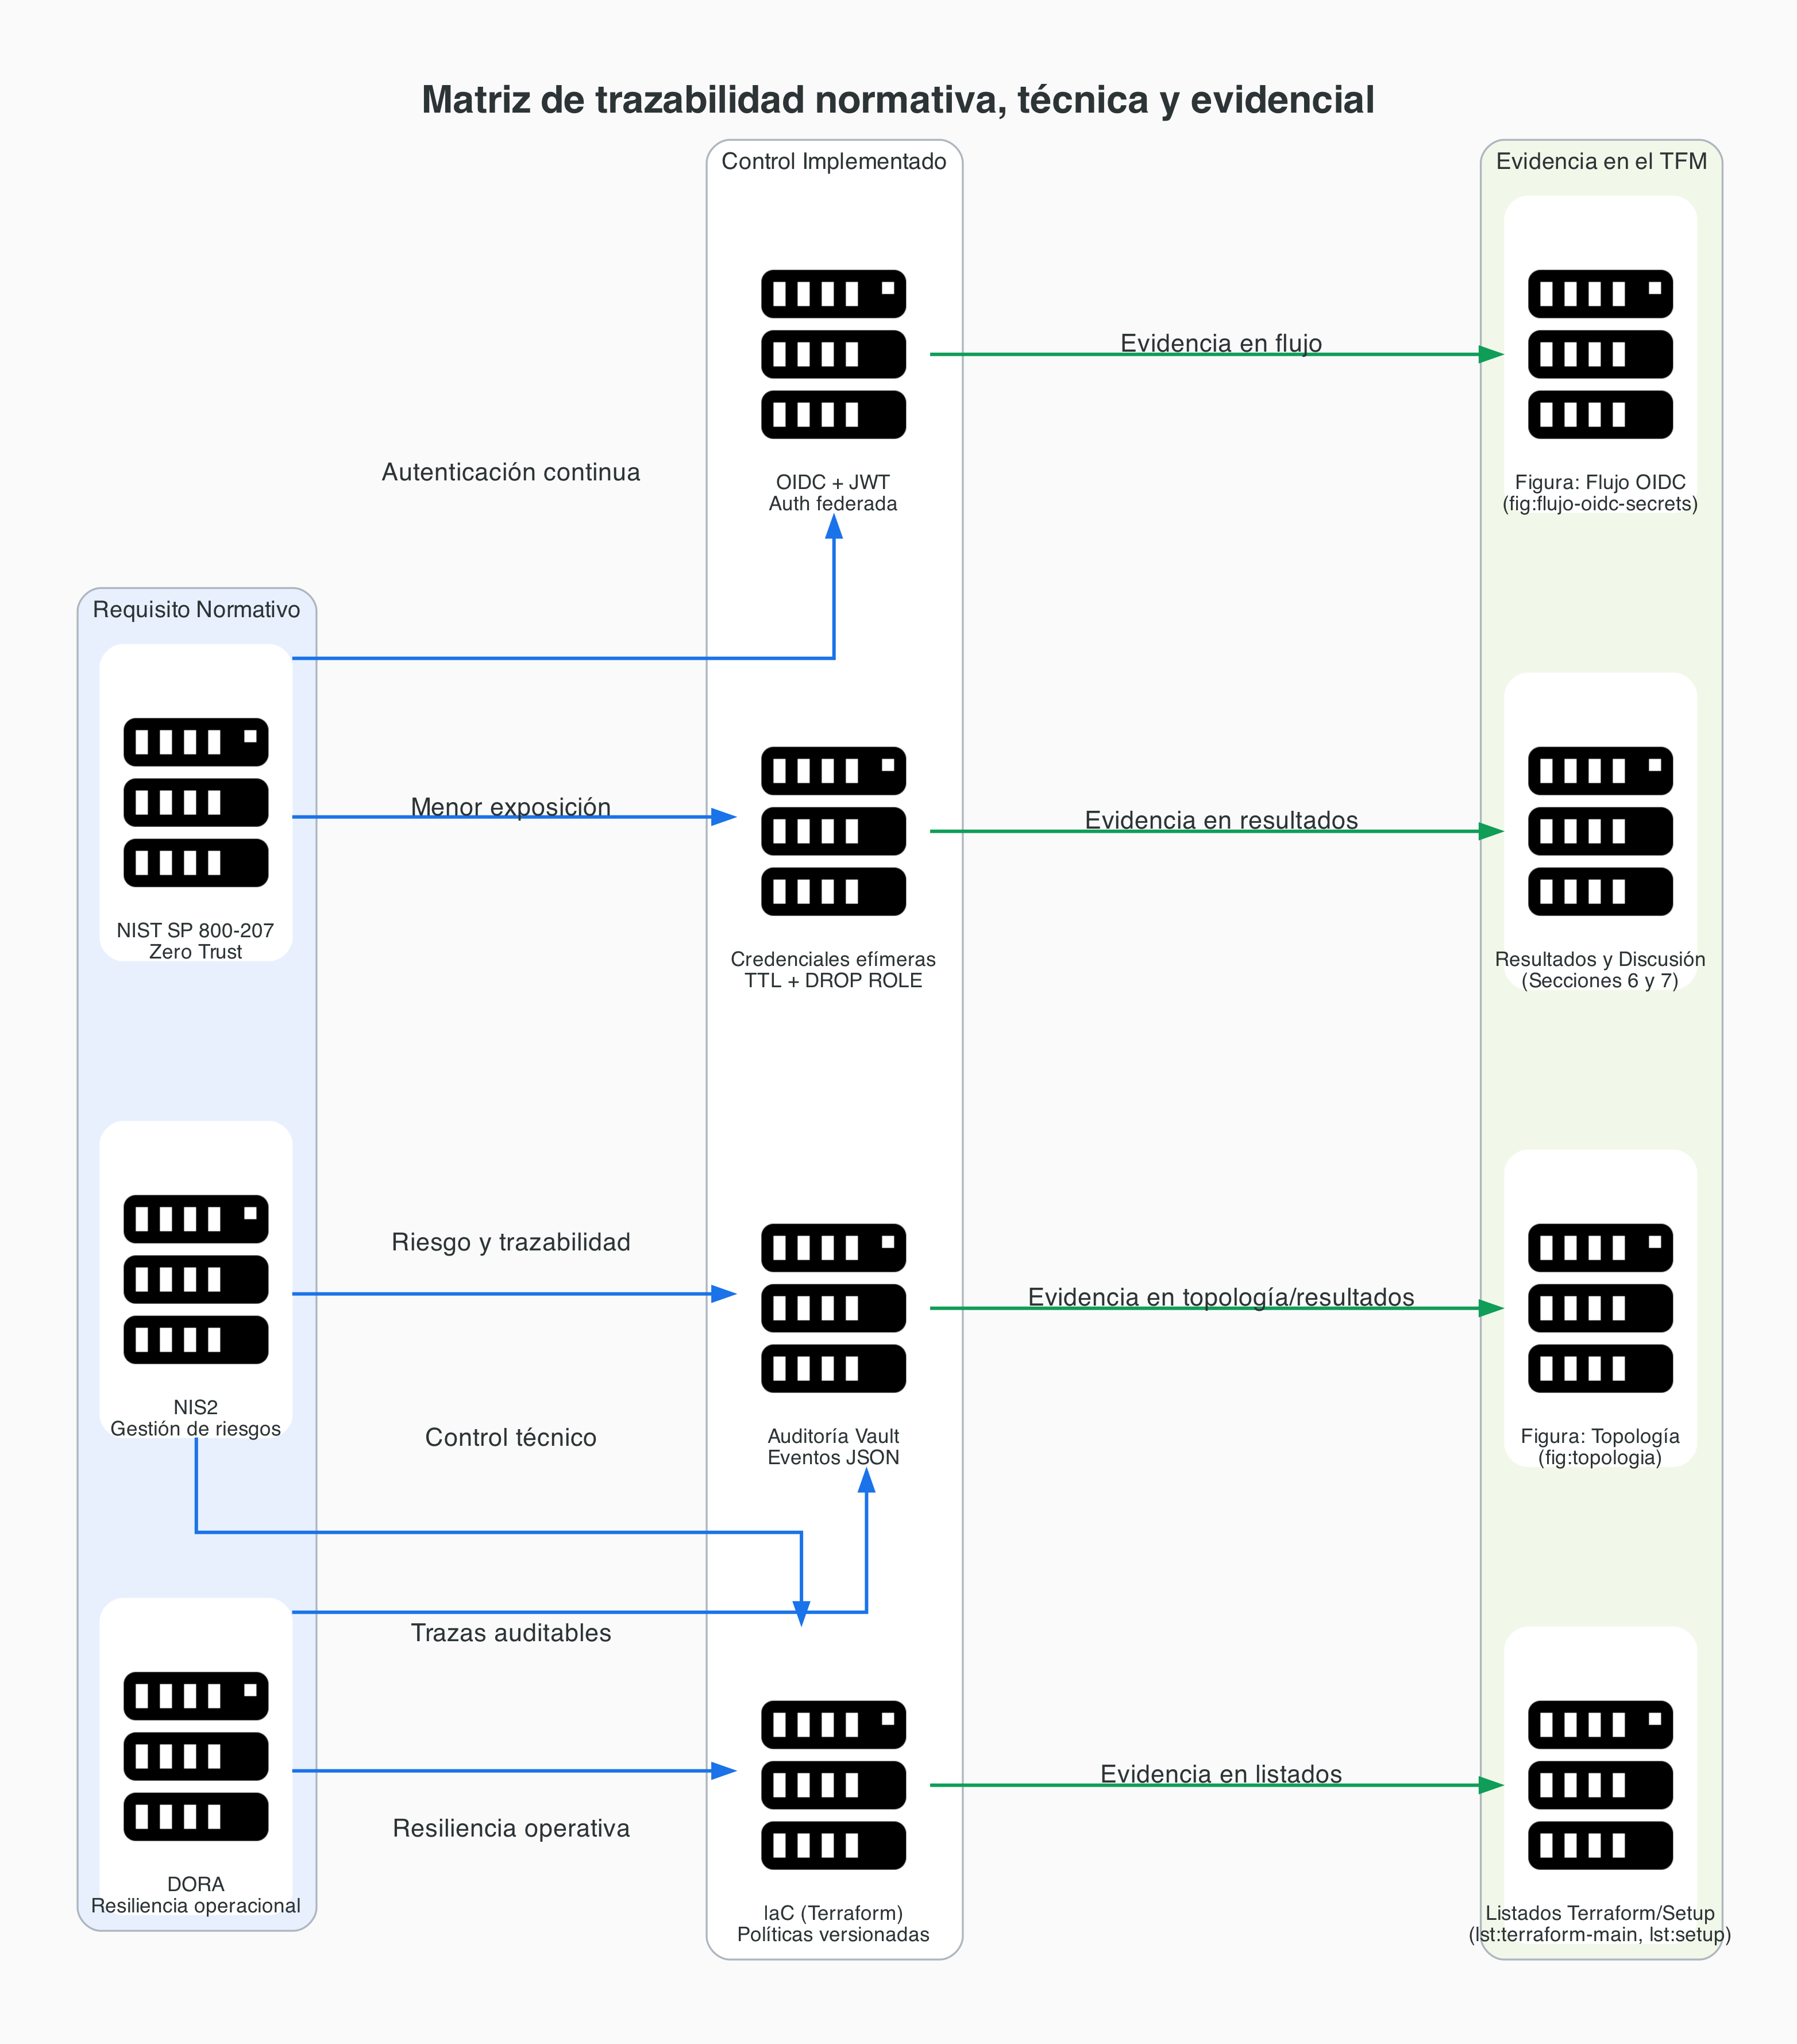
\includegraphics[width=\textwidth]{diagrams/matriz_trazabilidad.png}
    \caption{Matriz de trazabilidad entre requisitos normativos (NIST SP 800-207, NIS2 y DORA), controles implementados en la arquitectura y evidencias documentadas en el TFM.}
    \label{fig:matriz-trazabilidad}
\end{figure}

\subsection{Confirmación de hipótesis y relación con el Secret Sprawl}
Los resultados observados en el laboratorio respaldan la hipótesis principal: la sustitución de credenciales estáticas por emisión dinámica reduce el tiempo durante el cual una credencial podría reutilizarse tras una potencial exposición, mitigando \gls{secretsprawl}. Además, la trazabilidad habilitada en \gls{vault} y la arquitectura orientada a prevención son coherentes con buenas prácticas de secret management y secret scanning \parencite{owasp_secrets_management_cheat_sheet,github_secret_scanning,vault_audit_devices}.

\subsection{Amenazas a la validez y limitaciones}
Como limitación, el estudio se basa en un entorno de laboratorio on-premise con componentes específicos (Proxmox, \gls{lxc}, \gls{k3s}, \gls{vault} y PostgreSQL). La validez externa queda condicionada por la replicabilidad de la configuración y por la calidad de las políticas implementadas. Además, la medición cuantitativa (p. ej., latencias, distribución estadística de tiempos de emisión/revocación o tasa de falsos positivos en detección) no se detalla en esta versión del TFM, por lo que la evaluación se centra en evidencia funcional y trazabilidad operacional.


\subsection{Trabajo futuro}
Como trabajo futuro se recomienda ampliar el conjunto de pruebas con escenarios de fallo (p. ej., denegaciones por políticas, roturas de validación \gls{oidc}, fallos transitorios del motor de auditoría), incorporar métricas cuantitativas del pipeline y realizar correlación real de eventos hacia un sistema de monitorización tipo \gls{siem}. También sería deseable evaluar otras superficies de secretos (certificados, llaves de cifrado, credenciales de servicios) para generalizar el impacto de la arquitectura propuesta \parencite{vault_audit_devices}.

\section{Conclusiones}
La implementación y evaluación del laboratorio \textit{on-premise} demuestra la viabilidad técnica de erradicar los secretos estáticos en infraestructuras locales con altos requisitos de aislamiento.

La integración de una bóveda criptográfica centralizada, combinada con la federación de identidades \gls{oidc}, resuelve eficazmente el problema del "secreto cero" sin comprometer la automatización del ciclo \gls{cicd}. Se confirma que abstraer la gestión de acceso a través de herramientas de Infraestructura como Código (\gls{iac}) no solo acota la superficie de exposición ante exfiltraciones, sino que dota al equipo de ingeniería de una operativa ágil y puramente declarativa.

En conclusión, desplazar la seguridad hacia las fases iniciales del desarrollo (\textit{shift-left}) y basar el acceso en validaciones dinámicas de identidad transforma la postura defensiva de la organización, mitigando de forma medible la problemática del \gls{secretsprawl} y preparando la infraestructura para futuras adopciones de nubes híbridas.

\section{Glosario}
\glsaddall
\printglossaries

\newpage
\section{Bibliografía}
\printbibliography

\end{document}
